\documentclass[12pt, a4paper]{article}

\usepackage{graphicx}
\usepackage{float}
\usepackage{hyperref}
\usepackage{siunitx}
\usepackage{amsmath}

\begin{document}
	\pagenumbering{gobble}
		\begin{titlepage}
			\centering
			{\LARGE Controls Systems Practical 4 \par}
			\vspace*{1.5cm}
			{\large Q. Kruger, 216008466 \par}
			{\large R. de Bruyn, 216054484 \par}
			\vspace*{1.2cm}
			{\large \today}
			\vspace*{\fill}
			% 
\includegraphics[width=\textwidth]{img/UJ.jpg}
			\vspace*{\fill}
		\end{titlepage}

		\pagenumbering{roman}
		\tableofcontents
		\listoffigures
		\newpage
		\pagenumbering{arabic}

	\section{Prelab} % (fold)
	\label{sec:prelab}
		\subsection{Question 1a} % (fold)
		\label{sub:question_1a}
		The transfer function of interest is 

		\begin{equation}
			\label{eqn:G_1}
			G_1(s) =\frac{25}{s^2 +4s+25} \\
		\end{equation}
				
	
		This equation shows that the natural frequency $\omega_n$ is given as $\omega_n = 5$ and zeta is given as $\zeta = 0.8$\\ 

		Using the value for $\zeta$ and $\omega_n$ the rise time ($T_r$), settling time ($T_s$), peak time ($T_p$) and persent overshoot ($\%OS$)can be found using the respective equations:
		\[
			\begin{array}{rcl}

				T_r &=& \frac{1}{\omega_n}(1.763\zeta^3-0.147\zeta^2+1.039\zeta+1)\\
				T_s &=& \frac{4}{\zeta\omega_n}\\
				T_p &=& \frac{\pi}{\omega_n\sqrt{1-\zeta^2}}\\
				\%OS &=& e^{-(\frac{\zeta\pi}{\sqrt{1-\zeta^2}})} \times 100\\
				\\
				T_r &=& 0.493 s \\
				T_p &=& 1.05 s\\
				T_s &=& 1 s\\
				\%OS &=& 1.5 \%\\
			\end{array}
		\]

		The pole plot for the transfer function as given by equation \ref{eqn:G_1} is shown in Figure \ref{fig:pole_plot_pre_g1a} below

		\begin{figure}[H]
			\centering
				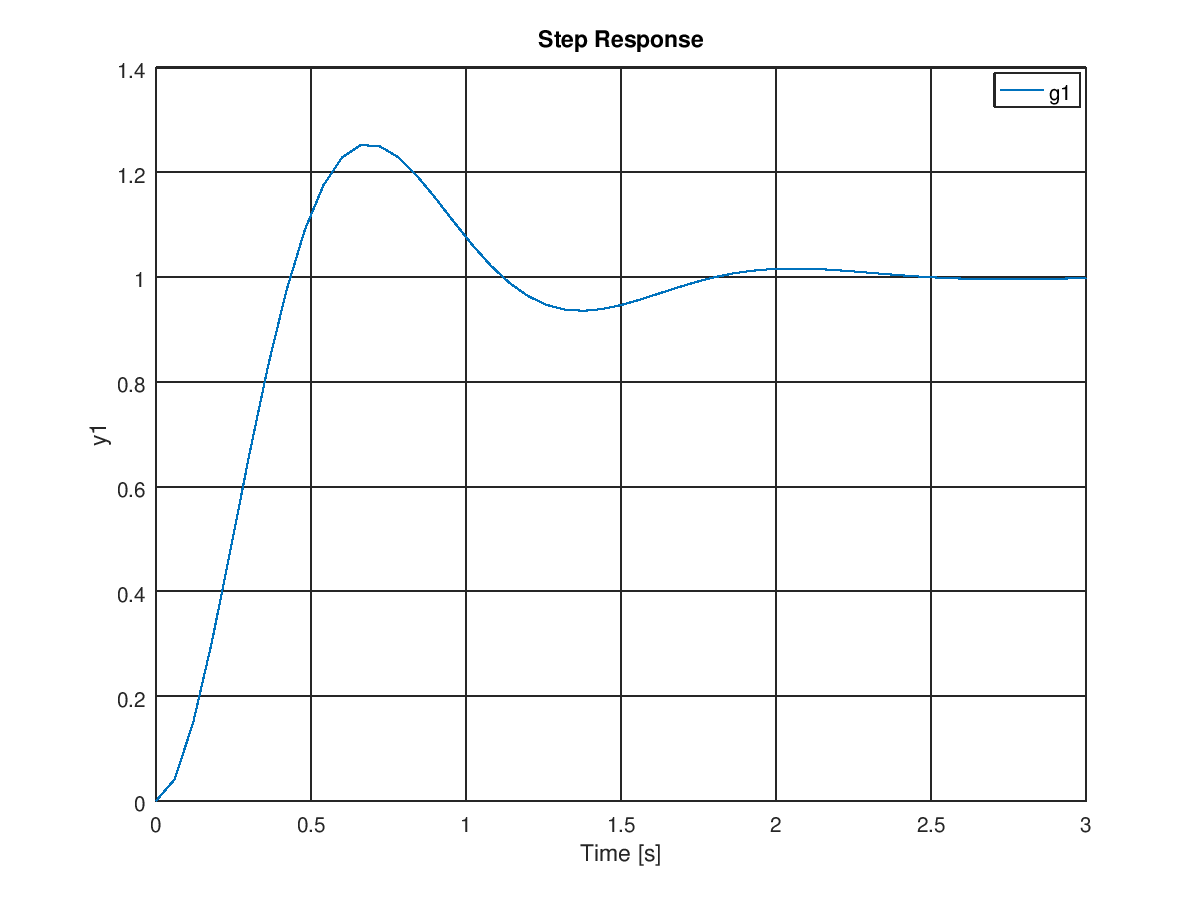
\includegraphics[width=0.7\textwidth]{Images/pole_plot_pre_q1a.png}
				\caption{Pole plot for $G_1$}
				\label{fig:pole_plot_pre_g1a} 
		\end{figure}
		% subsection question_1a (end)

		\subsection{Question 1b} % (fold)
		\label{sub:question_1b}
			Consider an additional pole at $s=-200$. The new transfer function is given shown by equation \eqref{eqn:G_2}
			\begin{equation}
				G_2 = \frac{25}{s^3+204s^2+825s+5000}
				\label{eqn:G_2}
			\end{equation}

			Comparing the transfer function $G_1$ with that of $G_2$, and normalizing $G_2$(by multiplying the transfer function $G_2$ with $200$) shows that the original system is not appreciably influenced by the addition of a system pole, as can be seen from figure below (Figure \ref{fig:step_pre_q1b}). 

			\begin{figure}[H]
				\centering
				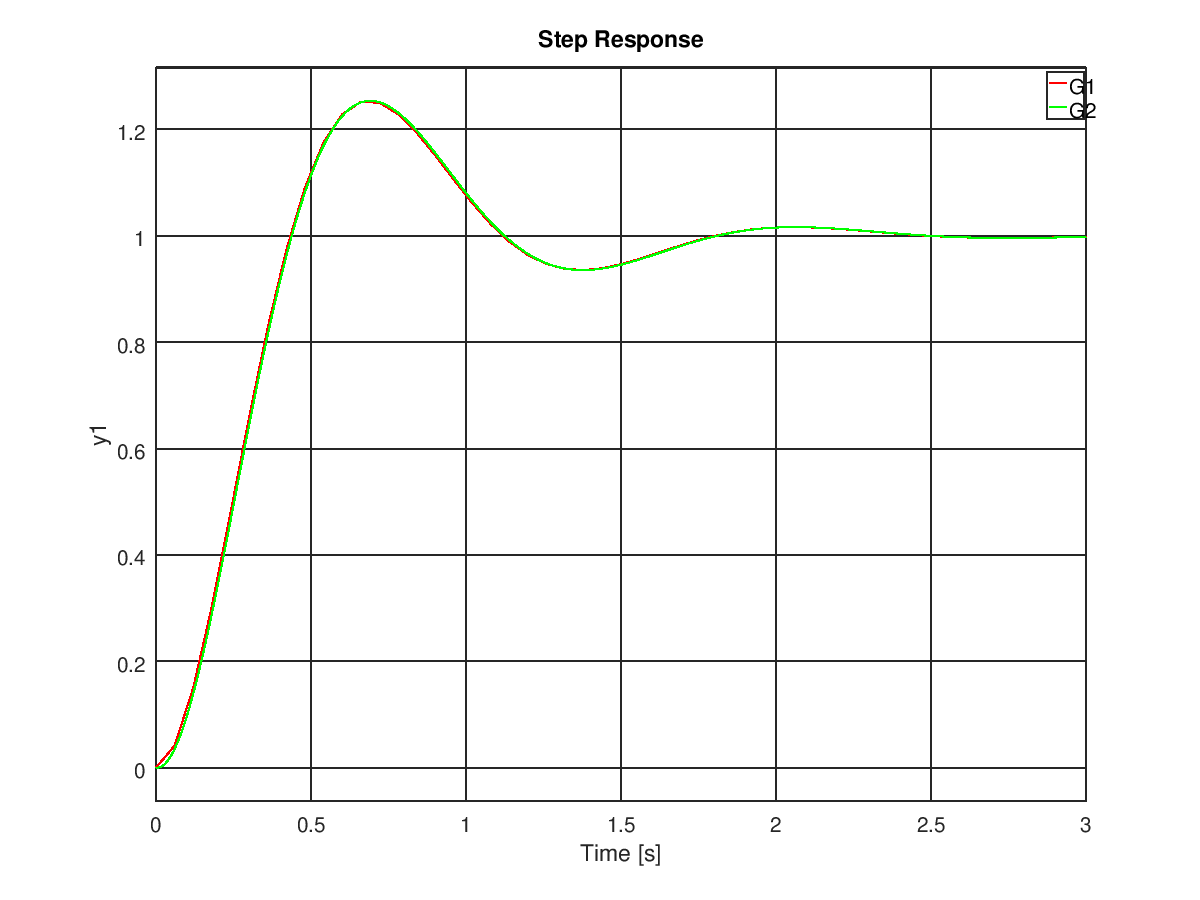
\includegraphics[width=0.7\textwidth]{Images/step_pre_q1b.png}
				\caption{Step response of the systems with transfer functions $G_1$ and $G_2$}
				\label{fig:step_pre_q1b}
			\end{figure}

			The rise time, settling time, peak time and percent overshoot of $G_2$ is similar to that of $G_1$.
		% subsection question_1b (end)

		\subsection{Question 1c} % (fold)
		\label{sub:question_1c}
			Consider the transfer functions corresponding to an addition of different poles at $s=-20$, $s=-10$ and $s=-2$ and normalized respectively
			\begin{equation}
				G_3 = \frac{20 \times 25}{s^3 +24s^2+105s+500}
			\end{equation}

			\begin{equation}
				G_4 = \frac{10 \times 25}{s^3 +14s^2+65s+250}
			\end{equation}

			\begin{equation}
				G_5 = \frac{2 \times 25}{s^3 +6s^2+33s+50}
			\end{equation}

			The plot of these step responses are shown in Figure \ref{fig:step_pre_q1c}
			\begin{figure}[H]
				\centering
				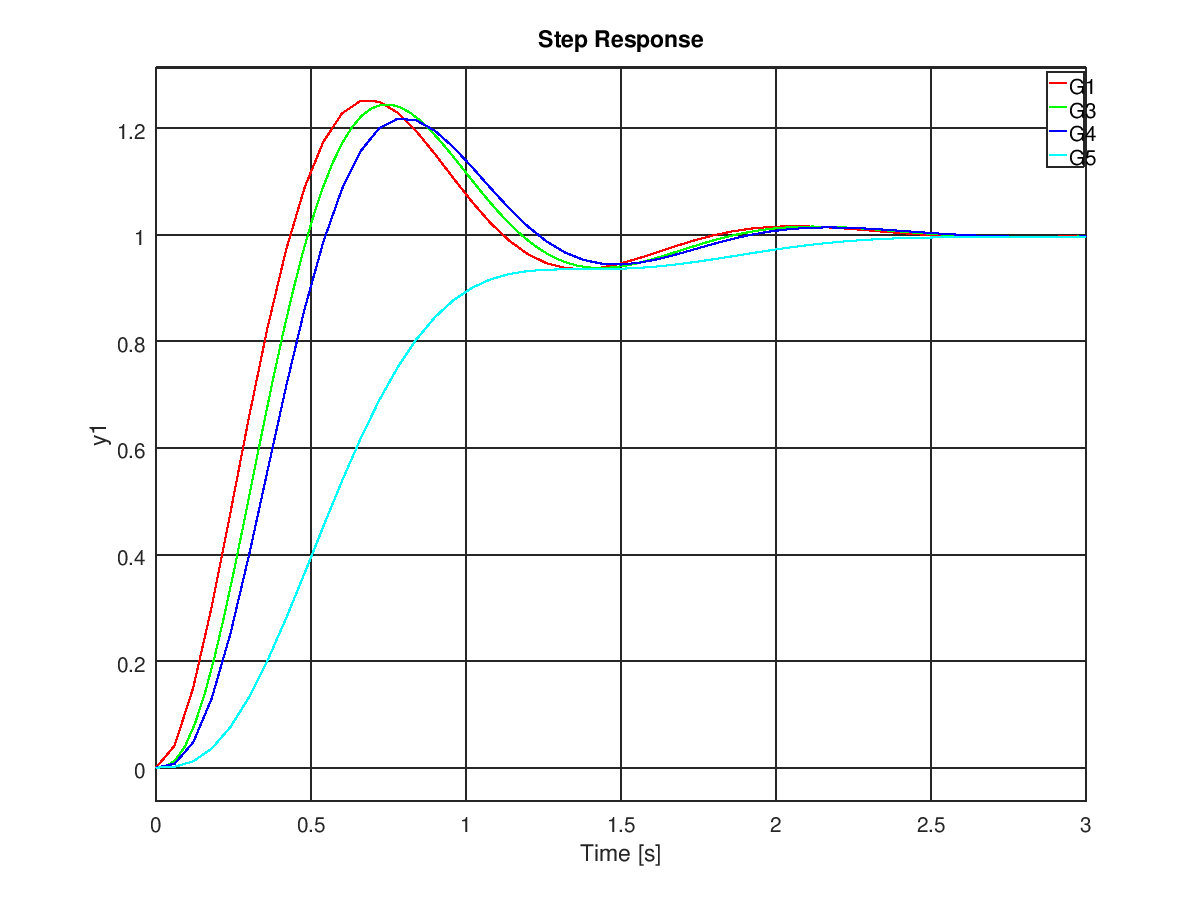
\includegraphics[width=0.7\textwidth]{Images/step_pre_q1c.png}
				\caption{Step response of the systems with transfer functions $G_1$, $G_3$, $G_4$ and $G_5$}
				\label{fig:step_pre_q1c}
			\end{figure}

			As can be seen from Figure \ref{fig:step_pre_q1c}, significant changes to the step response occurs when the addition of a system pole lies close to the imaginary axis

		% subsection question_1b (end)
			\subsection{Question 2} % (fold)
			\label{sub:question_2}
				Multiplying \eqref{eqn:G_1} with different zeros respectively at $s=-200$, $s=-50$,$s=-10$ and $s=-2$ gives us the new transfer functions given as shown below
				\begin{equation}
					G_6 = \frac{25s +5000}{s^2+4s+25}
					\label{eqn:G_6}
				\end{equation}

				\begin{equation}
					G_7 = \frac{25s +1250}{s^2+4s+25}
					\label{eqn:G_7}
				\end{equation}

				\begin{equation}
					G_8 = \frac{25s +250}{s^2+4s+25}
					\label{eqn:G_8}
				\end{equation}

				\begin{equation}
					G_9 = \frac{25s +50}{s^2+4s+25}
					\label{eqn:G_9}
				\end{equation}

				The step responses of these transfer functions are show below in Figure \ref{fig:step_pre_2}

				\begin{figure}[H]
					\centering
					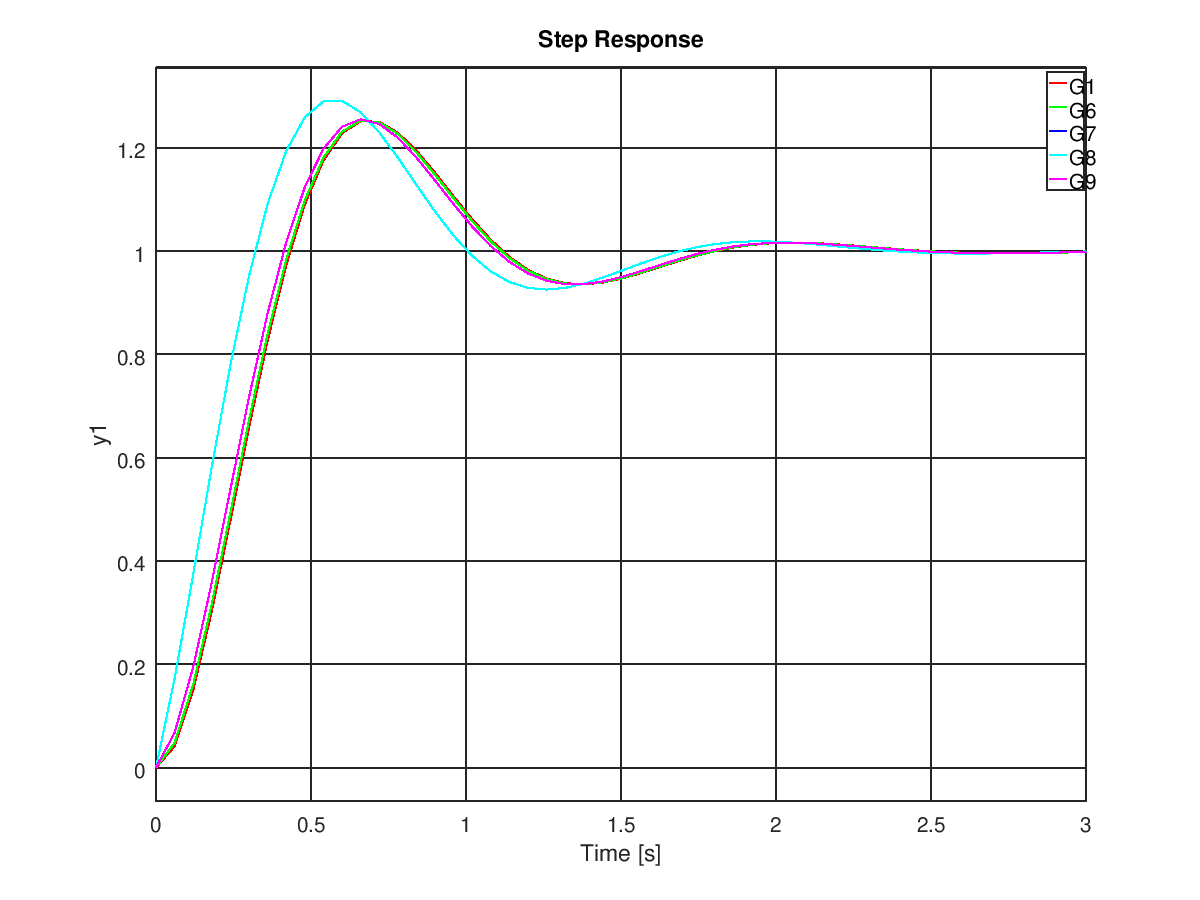
\includegraphics[width=0.7\textwidth]{Images/step_pre_2.png}
					\caption{Step response of the systems with transfer functions $G_1$, $G_6$, $G_7$, $G_8$ and $G_9$}
					\label{fig:step_pre_2}
				\end{figure}

				It is evident from Figure \ref{fig:step_pre_2} that as the zeros move farther away from the imaginary axis, so the effect it has on the system as described by equation \eqref{eqn:G_1} becomes greater. The values of the zeros with the greatest to the least effect on the system is listed below.
				\begin{enumerate}
	 				\item $s=-2$
	 				\item $s=-10$
	 				\item $s=-50$
	 				\item $s=-200$
	 			\end{enumerate}
			
			% subsection question_2 (end)

			\subsection{Question 3} % (fold)
			\label{sub:question_3}
			As was seen from question 1c of the prelab section, the further away the pole from the imaginary axis, the less effect it has on the second order system. Thus given the values for $b$ (given the additional pole as $s+b$), the value $4$ would mean that the pole $s+b$ has minimal effect upon the second-order transient response	
			% subsection question_3 (end)

			\subsection{Question 4} % (fold)
			\label{sub:question_4}
			Once again, the value of $b$ corresponding to a pole location the furthest away from the imaginary axis is the value $b=40$ thus the pole corresponding to this value of $b$ is $s=-40$. This value of $b$ makes the effect of the pole on the system the smallest of all the other values of $b$.
			
			% subsection question_4 (end)

	\section{Lab} % (fold)
	\label{sec:lab}
	Making use of MATLAB's \texttt{stepinfo} function we were able to obtain the step response information relevant to the addition of a zeros at the respective locations at $s=-200$, $s=-50$, $s=-10$, $s=-2$. The transfer functions corresponding to these zeros are those of prelab question 1b and question 1c ($G_2$-$G_5$).

	The information for the respective transfer functions are given as:

	\begin{enumerate}
		\item For $G_6$ \\
		Rise Time: 0.2928 \\
		Settling Time: 1.6769 \\
		Settling Min: 0.9187 \\
		Settling Max: 1.2536 \\
		Oversjoot: 25.3577 \\
		Undershoot: 0 \\
		Peak: 1.2536 \\
		Peak Time: 0.6908 \\

		\item For $G_7$ \\
		Rise Time: 0.2909 \\
		Settling Time: 1.6617 \\
		Settling Min: 0.9005 \\
		Settling Max: 1.2551 \\
		Oversjoot: 25.5136 \\
		Undershoot: 0 \\
		Peak: 1.2551 \\
		Peak Time: 0.6677 \\

		\item For $G_8$ \\
		Rise Time: 0.2448 \\
		Settling Time: 1.5831 \\
		Settling Min: 0.9255 \\
		Settling Max: 1.2936 \\
		Oversjoot: 29.3613 \\
		Undershoot: 0 \\
		Peak: 1.2936 \\
		Peak Time: 0.5756 \\

		\item For $G_9$ \\
		Rise Time: 0.0716 \\
		Settling Time: 2.0247 \\
		Settling Min: 0.7072 \\
		Settling Max: 2.1543 \\
		Oversjoot: 115.4281 \\
		Undershoot: 0 \\
		Peak: 2.1543 \\
		Peak Time: 0.3454 \\
		
	\end{enumerate}




	
	
	% section lab (end)

	\section{Post Lab} % (fold)
	\label{sec:post_lab}
	As was mentioned in the prelab section of this report, as the additional pole moves closer to the dominant pole, the step response drastically gets influeced as can be seen from Figure \ref{fig:step_pre_q1c} of the prelab.
	
	% section post_lab (end)

			
	% section prelab (end)

\end{document}

